% Options for packages loaded elsewhere
\PassOptionsToPackage{unicode}{hyperref}
\PassOptionsToPackage{hyphens}{url}
%
\documentclass[
]{article}
\usepackage{lmodern}
\usepackage{amssymb,amsmath}
\usepackage{ifxetex,ifluatex}
\ifnum 0\ifxetex 1\fi\ifluatex 1\fi=0 % if pdftex
  \usepackage[T1]{fontenc}
  \usepackage[utf8]{inputenc}
  \usepackage{textcomp} % provide euro and other symbols
\else % if luatex or xetex
  \usepackage{unicode-math}
  \defaultfontfeatures{Scale=MatchLowercase}
  \defaultfontfeatures[\rmfamily]{Ligatures=TeX,Scale=1}
\fi
% Use upquote if available, for straight quotes in verbatim environments
\IfFileExists{upquote.sty}{\usepackage{upquote}}{}
\IfFileExists{microtype.sty}{% use microtype if available
  \usepackage[]{microtype}
  \UseMicrotypeSet[protrusion]{basicmath} % disable protrusion for tt fonts
}{}
\makeatletter
\@ifundefined{KOMAClassName}{% if non-KOMA class
  \IfFileExists{parskip.sty}{%
    \usepackage{parskip}
  }{% else
    \setlength{\parindent}{0pt}
    \setlength{\parskip}{6pt plus 2pt minus 1pt}}
}{% if KOMA class
  \KOMAoptions{parskip=half}}
\makeatother
\usepackage{xcolor}
\IfFileExists{xurl.sty}{\usepackage{xurl}}{} % add URL line breaks if available
\IfFileExists{bookmark.sty}{\usepackage{bookmark}}{\usepackage{hyperref}}
\hypersetup{
  hidelinks,
  pdfcreator={LaTeX via pandoc}}
\urlstyle{same} % disable monospaced font for URLs
\usepackage[margin=1in]{geometry}
\usepackage{color}
\usepackage{fancyvrb}
\newcommand{\VerbBar}{|}
\newcommand{\VERB}{\Verb[commandchars=\\\{\}]}
\DefineVerbatimEnvironment{Highlighting}{Verbatim}{commandchars=\\\{\}}
% Add ',fontsize=\small' for more characters per line
\usepackage{framed}
\definecolor{shadecolor}{RGB}{248,248,248}
\newenvironment{Shaded}{\begin{snugshade}}{\end{snugshade}}
\newcommand{\AlertTok}[1]{\textcolor[rgb]{0.94,0.16,0.16}{#1}}
\newcommand{\AnnotationTok}[1]{\textcolor[rgb]{0.56,0.35,0.01}{\textbf{\textit{#1}}}}
\newcommand{\AttributeTok}[1]{\textcolor[rgb]{0.77,0.63,0.00}{#1}}
\newcommand{\BaseNTok}[1]{\textcolor[rgb]{0.00,0.00,0.81}{#1}}
\newcommand{\BuiltInTok}[1]{#1}
\newcommand{\CharTok}[1]{\textcolor[rgb]{0.31,0.60,0.02}{#1}}
\newcommand{\CommentTok}[1]{\textcolor[rgb]{0.56,0.35,0.01}{\textit{#1}}}
\newcommand{\CommentVarTok}[1]{\textcolor[rgb]{0.56,0.35,0.01}{\textbf{\textit{#1}}}}
\newcommand{\ConstantTok}[1]{\textcolor[rgb]{0.00,0.00,0.00}{#1}}
\newcommand{\ControlFlowTok}[1]{\textcolor[rgb]{0.13,0.29,0.53}{\textbf{#1}}}
\newcommand{\DataTypeTok}[1]{\textcolor[rgb]{0.13,0.29,0.53}{#1}}
\newcommand{\DecValTok}[1]{\textcolor[rgb]{0.00,0.00,0.81}{#1}}
\newcommand{\DocumentationTok}[1]{\textcolor[rgb]{0.56,0.35,0.01}{\textbf{\textit{#1}}}}
\newcommand{\ErrorTok}[1]{\textcolor[rgb]{0.64,0.00,0.00}{\textbf{#1}}}
\newcommand{\ExtensionTok}[1]{#1}
\newcommand{\FloatTok}[1]{\textcolor[rgb]{0.00,0.00,0.81}{#1}}
\newcommand{\FunctionTok}[1]{\textcolor[rgb]{0.00,0.00,0.00}{#1}}
\newcommand{\ImportTok}[1]{#1}
\newcommand{\InformationTok}[1]{\textcolor[rgb]{0.56,0.35,0.01}{\textbf{\textit{#1}}}}
\newcommand{\KeywordTok}[1]{\textcolor[rgb]{0.13,0.29,0.53}{\textbf{#1}}}
\newcommand{\NormalTok}[1]{#1}
\newcommand{\OperatorTok}[1]{\textcolor[rgb]{0.81,0.36,0.00}{\textbf{#1}}}
\newcommand{\OtherTok}[1]{\textcolor[rgb]{0.56,0.35,0.01}{#1}}
\newcommand{\PreprocessorTok}[1]{\textcolor[rgb]{0.56,0.35,0.01}{\textit{#1}}}
\newcommand{\RegionMarkerTok}[1]{#1}
\newcommand{\SpecialCharTok}[1]{\textcolor[rgb]{0.00,0.00,0.00}{#1}}
\newcommand{\SpecialStringTok}[1]{\textcolor[rgb]{0.31,0.60,0.02}{#1}}
\newcommand{\StringTok}[1]{\textcolor[rgb]{0.31,0.60,0.02}{#1}}
\newcommand{\VariableTok}[1]{\textcolor[rgb]{0.00,0.00,0.00}{#1}}
\newcommand{\VerbatimStringTok}[1]{\textcolor[rgb]{0.31,0.60,0.02}{#1}}
\newcommand{\WarningTok}[1]{\textcolor[rgb]{0.56,0.35,0.01}{\textbf{\textit{#1}}}}
\usepackage{graphicx,grffile}
\makeatletter
\def\maxwidth{\ifdim\Gin@nat@width>\linewidth\linewidth\else\Gin@nat@width\fi}
\def\maxheight{\ifdim\Gin@nat@height>\textheight\textheight\else\Gin@nat@height\fi}
\makeatother
% Scale images if necessary, so that they will not overflow the page
% margins by default, and it is still possible to overwrite the defaults
% using explicit options in \includegraphics[width, height, ...]{}
\setkeys{Gin}{width=\maxwidth,height=\maxheight,keepaspectratio}
% Set default figure placement to htbp
\makeatletter
\def\fps@figure{htbp}
\makeatother
\setlength{\emergencystretch}{3em} % prevent overfull lines
\providecommand{\tightlist}{%
  \setlength{\itemsep}{0pt}\setlength{\parskip}{0pt}}
\setcounter{secnumdepth}{-\maxdimen} % remove section numbering

\title{Prácticas de Estadística\\
Ejercicio de la Práctica 2\\
Variable Aleatoria}
\author{true}
\date{Versión 22-diciembre-2020}

\begin{document}
\maketitle

{
\setcounter{tocdepth}{2}
\tableofcontents
}
\hypertarget{primer-ejercicio}{%
\section{Primer ejercicio}\label{primer-ejercicio}}

Consideremos una variable aleatoria, \(X\) que sigue una distribución
\(B(15, 0.33)\). Se pide:

\begin{enumerate}
\def\labelenumi{\arabic{enumi}.}
\tightlist
\item
  Calcular:
\end{enumerate}

\begin{itemize}
\tightlist
\item
  \(P[4\leq X \leq 8]\).
\end{itemize}

\begin{Shaded}
\begin{Highlighting}[]
\CommentTok{# Responde aquí}
\KeywordTok{sum}\NormalTok{(}\KeywordTok{dbinom}\NormalTok{(}\DecValTok{4}\OperatorTok{:}\DecValTok{8}\NormalTok{,}\DecValTok{15}\NormalTok{,}\FloatTok{0.33}\NormalTok{))}
\end{Highlighting}
\end{Shaded}

\begin{verbatim}
## [1] 0.7540009
\end{verbatim}

\begin{itemize}
\tightlist
\item
  \(P[4 < X \leq 8]\).
\end{itemize}

\begin{Shaded}
\begin{Highlighting}[]
\CommentTok{# Responde aquí}
\KeywordTok{sum}\NormalTok{(}\KeywordTok{dbinom}\NormalTok{(}\DecValTok{5}\OperatorTok{:}\DecValTok{8}\NormalTok{,}\DecValTok{15}\NormalTok{,}\FloatTok{0.33}\NormalTok{))}
\end{Highlighting}
\end{Shaded}

\begin{verbatim}
## [1] 0.5562988
\end{verbatim}

\begin{itemize}
\tightlist
\item
  \(P[4 < X < 8]\).
\end{itemize}

\begin{Shaded}
\begin{Highlighting}[]
\CommentTok{# Responde aquí}
\KeywordTok{sum}\NormalTok{(}\KeywordTok{dbinom}\NormalTok{(}\DecValTok{5}\OperatorTok{:}\DecValTok{7}\NormalTok{,}\DecValTok{15}\NormalTok{,}\FloatTok{0.33}\NormalTok{))}
\end{Highlighting}
\end{Shaded}

\begin{verbatim}
## [1] 0.5014479
\end{verbatim}

\begin{itemize}
\tightlist
\item
  \(P[X \geq 4]\).
\end{itemize}

\begin{Shaded}
\begin{Highlighting}[]
\CommentTok{# Responde aquí}
\KeywordTok{sum}\NormalTok{(}\KeywordTok{dbinom}\NormalTok{(}\DecValTok{4}\OperatorTok{:}\DecValTok{15}\NormalTok{,}\DecValTok{15}\NormalTok{,}\FloatTok{0.33}\NormalTok{))}
\end{Highlighting}
\end{Shaded}

\begin{verbatim}
## [1] 0.7828694
\end{verbatim}

\begin{itemize}
\tightlist
\item
  \(P[X > 4]\).
\end{itemize}

\begin{Shaded}
\begin{Highlighting}[]
\CommentTok{# Responde aquí}
\KeywordTok{sum}\NormalTok{(}\KeywordTok{dbinom}\NormalTok{(}\DecValTok{5}\OperatorTok{:}\DecValTok{15}\NormalTok{,}\DecValTok{15}\NormalTok{,}\FloatTok{0.33}\NormalTok{))}
\end{Highlighting}
\end{Shaded}

\begin{verbatim}
## [1] 0.5851673
\end{verbatim}

\begin{enumerate}
\def\labelenumi{\arabic{enumi}.}
\setcounter{enumi}{1}
\tightlist
\item
  Obtener:
\end{enumerate}

\begin{itemize}
\tightlist
\item
  El primer valor de la variable que deja por debajo de sí al menos el
  95\% de la probabilidad:
\end{itemize}

\begin{Shaded}
\begin{Highlighting}[]
\CommentTok{# Responde aquí}
\KeywordTok{qbinom}\NormalTok{(}\FloatTok{0.95}\NormalTok{,}\DecValTok{15}\NormalTok{,}\FloatTok{0.33}\NormalTok{)}
\end{Highlighting}
\end{Shaded}

\begin{verbatim}
## [1] 8
\end{verbatim}

\begin{itemize}
\tightlist
\item
  El percentil 95 de la distribución.
\end{itemize}

\begin{Shaded}
\begin{Highlighting}[]
\CommentTok{# Responde aquí}
\KeywordTok{qbinom}\NormalTok{(}\FloatTok{0.95}\NormalTok{,}\DecValTok{15}\NormalTok{,}\FloatTok{0.33}\NormalTok{)}
\end{Highlighting}
\end{Shaded}

\begin{verbatim}
## [1] 8
\end{verbatim}

\begin{enumerate}
\def\labelenumi{\arabic{enumi}.}
\setcounter{enumi}{2}
\tightlist
\item
  Obtener una muestra de tamaño 10 de esta distribución
\end{enumerate}

\begin{Shaded}
\begin{Highlighting}[]
\CommentTok{# Responde aquí}
\KeywordTok{rbinom}\NormalTok{(}\DecValTok{10}\NormalTok{,}\DecValTok{15}\NormalTok{,}\FloatTok{0.33}\NormalTok{)}
\end{Highlighting}
\end{Shaded}

\begin{verbatim}
##  [1] 6 5 5 4 7 5 6 7 6 3
\end{verbatim}

\hypertarget{segundo-ejercicio}{%
\section{Segundo ejercicio}\label{segundo-ejercicio}}

Consideremos una variable aleatoria que sigue una distribución
\(Poisson(7.2)\). Se pide:

\begin{enumerate}
\def\labelenumi{\arabic{enumi}.}
\tightlist
\item
  Calcular:
\end{enumerate}

\begin{itemize}
\tightlist
\item
  \(P[X > 5]\).
\end{itemize}

\begin{Shaded}
\begin{Highlighting}[]
\CommentTok{# Responde aquí}
\DecValTok{1}\OperatorTok{-}\KeywordTok{sum}\NormalTok{(}\KeywordTok{dpois}\NormalTok{(}\DecValTok{0}\OperatorTok{:}\DecValTok{5}\NormalTok{,}\FloatTok{7.2}\NormalTok{))}
\end{Highlighting}
\end{Shaded}

\begin{verbatim}
## [1] 0.7241025
\end{verbatim}

\begin{itemize}
\tightlist
\item
  \(P[X \geq 5]\).
\end{itemize}

\begin{Shaded}
\begin{Highlighting}[]
\CommentTok{# Responde aquí}
\DecValTok{1}\OperatorTok{-}\KeywordTok{sum}\NormalTok{(}\KeywordTok{dpois}\NormalTok{(}\DecValTok{0}\OperatorTok{:}\DecValTok{4}\NormalTok{,}\FloatTok{7.2}\NormalTok{))}
\end{Highlighting}
\end{Shaded}

\begin{verbatim}
## [1] 0.8444844
\end{verbatim}

\begin{itemize}
\tightlist
\item
  \(P[2 < X < 8]\).
\end{itemize}

\begin{Shaded}
\begin{Highlighting}[]
\CommentTok{# Responde aquí}
\KeywordTok{sum}\NormalTok{(}\KeywordTok{dpois}\NormalTok{(}\DecValTok{3}\OperatorTok{:}\DecValTok{7}\NormalTok{,}\FloatTok{7.2}\NormalTok{))}
\end{Highlighting}
\end{Shaded}

\begin{verbatim}
## [1] 0.5434677
\end{verbatim}

\begin{itemize}
\tightlist
\item
  \(P[2 \leq X < 8]\).
\end{itemize}

\begin{Shaded}
\begin{Highlighting}[]
\CommentTok{# Responde aquí}
\KeywordTok{sum}\NormalTok{(}\KeywordTok{dpois}\NormalTok{(}\DecValTok{2}\OperatorTok{:}\DecValTok{7}\NormalTok{,}\FloatTok{7.2}\NormalTok{))}
\end{Highlighting}
\end{Shaded}

\begin{verbatim}
## [1] 0.5628192
\end{verbatim}

\begin{itemize}
\tightlist
\item
  \(P[2 < X \leq 8]\).
\end{itemize}

\begin{Shaded}
\begin{Highlighting}[]
\CommentTok{# Responde aquí}
\KeywordTok{sum}\NormalTok{(}\KeywordTok{dpois}\NormalTok{(}\DecValTok{3}\OperatorTok{:}\DecValTok{8}\NormalTok{,}\FloatTok{7.2}\NormalTok{))}
\end{Highlighting}
\end{Shaded}

\begin{verbatim}
## [1] 0.6771948
\end{verbatim}

\begin{itemize}
\tightlist
\item
  \(P[X < 7]\).
\end{itemize}

\begin{Shaded}
\begin{Highlighting}[]
\CommentTok{# Responde aquí}
\KeywordTok{sum}\NormalTok{(}\KeywordTok{dpois}\NormalTok{(}\DecValTok{0}\OperatorTok{:}\DecValTok{6}\NormalTok{,}\FloatTok{7.2}\NormalTok{))}
\end{Highlighting}
\end{Shaded}

\begin{verbatim}
## [1] 0.4203557
\end{verbatim}

\begin{itemize}
\tightlist
\item
  \(P[X \leq 7]\).
\end{itemize}

\begin{Shaded}
\begin{Highlighting}[]
\CommentTok{# Responde aquí}
\KeywordTok{sum}\NormalTok{(}\KeywordTok{dpois}\NormalTok{(}\DecValTok{0}\OperatorTok{:}\DecValTok{7}\NormalTok{,}\FloatTok{7.2}\NormalTok{))}
\end{Highlighting}
\end{Shaded}

\begin{verbatim}
## [1] 0.5689412
\end{verbatim}

\begin{itemize}
\tightlist
\item
  \(P[X = 7]\).
\end{itemize}

\begin{Shaded}
\begin{Highlighting}[]
\CommentTok{# Responde aquí}
\KeywordTok{sum}\NormalTok{(}\KeywordTok{dpois}\NormalTok{(}\DecValTok{7}\NormalTok{,}\FloatTok{7.2}\NormalTok{))}
\end{Highlighting}
\end{Shaded}

\begin{verbatim}
## [1] 0.1485856
\end{verbatim}

\begin{enumerate}
\def\labelenumi{\arabic{enumi}.}
\setcounter{enumi}{1}
\tightlist
\item
  Obtener:
\end{enumerate}

\begin{itemize}
\tightlist
\item
  El percentil 75 de la distribución.
\end{itemize}

\begin{Shaded}
\begin{Highlighting}[]
\CommentTok{# Responde aquí}
\KeywordTok{qpois}\NormalTok{(}\FloatTok{0.75}\NormalTok{,}\FloatTok{7.2}\NormalTok{)}
\end{Highlighting}
\end{Shaded}

\begin{verbatim}
## [1] 9
\end{verbatim}

\begin{itemize}
\tightlist
\item
  El primer valor de la variable que deja por debajo de sí al menos el
  5\% de sus valores.
\end{itemize}

\begin{Shaded}
\begin{Highlighting}[]
\CommentTok{# Responde aquí}
\KeywordTok{qpois}\NormalTok{(}\FloatTok{0.05}\NormalTok{,}\FloatTok{7.2}\NormalTok{)}
\end{Highlighting}
\end{Shaded}

\begin{verbatim}
## [1] 3
\end{verbatim}

\begin{enumerate}
\def\labelenumi{\arabic{enumi}.}
\setcounter{enumi}{2}
\tightlist
\item
  Obtener una muestra de tamaño 5 de la distribución.
\end{enumerate}

\begin{Shaded}
\begin{Highlighting}[]
\CommentTok{# Responde aquí}
\KeywordTok{rpois}\NormalTok{(}\DecValTok{5}\NormalTok{,}\FloatTok{7.2}\NormalTok{)}
\end{Highlighting}
\end{Shaded}

\begin{verbatim}
## [1]  4 10  4 11  5
\end{verbatim}

\hypertarget{tercer-ejercicio}{%
\section{Tercer ejercicio}\label{tercer-ejercicio}}

Consideremos una variable aleatoria \(X\) que sigue una distribución
exponencial \textbf{de media 2}. Se pide:

\begin{enumerate}
\def\labelenumi{\arabic{enumi}.}
\tightlist
\item
  Calcular:
\end{enumerate}

\begin{itemize}
\tightlist
\item
  \(P [X = 5]\).
\end{itemize}

\begin{Shaded}
\begin{Highlighting}[]
\CommentTok{# Responde aquí}
\KeywordTok{pexp}\NormalTok{(}\DecValTok{5}\NormalTok{,}\DecValTok{1}\OperatorTok{/}\DecValTok{2}\NormalTok{)}\OperatorTok{-}\KeywordTok{pexp}\NormalTok{(}\DecValTok{5}\NormalTok{,}\DecValTok{1}\OperatorTok{/}\DecValTok{2}\NormalTok{)}
\end{Highlighting}
\end{Shaded}

\begin{verbatim}
## [1] 0
\end{verbatim}

\begin{itemize}
\tightlist
\item
  \(P [X \leq 5]\).
\end{itemize}

\begin{Shaded}
\begin{Highlighting}[]
\CommentTok{# Responde aquí}
\KeywordTok{pexp}\NormalTok{(}\DecValTok{5}\NormalTok{,}\DecValTok{1}\OperatorTok{/}\DecValTok{2}\NormalTok{)}
\end{Highlighting}
\end{Shaded}

\begin{verbatim}
## [1] 0.917915
\end{verbatim}

\begin{itemize}
\tightlist
\item
  \(P [X < 5]\).
\end{itemize}

\begin{Shaded}
\begin{Highlighting}[]
\CommentTok{# Responde aquí}
\KeywordTok{pexp}\NormalTok{(}\DecValTok{5}\NormalTok{,}\DecValTok{1}\OperatorTok{/}\DecValTok{2}\NormalTok{)}
\end{Highlighting}
\end{Shaded}

\begin{verbatim}
## [1] 0.917915
\end{verbatim}

\begin{itemize}
\tightlist
\item
  \(P [2 \leq X \leq 8]\).
\end{itemize}

\begin{Shaded}
\begin{Highlighting}[]
\CommentTok{# Responde aquí}
\KeywordTok{pexp}\NormalTok{(}\DecValTok{8}\NormalTok{,}\DecValTok{1}\OperatorTok{/}\DecValTok{2}\NormalTok{)}\OperatorTok{-}\KeywordTok{pexp}\NormalTok{(}\DecValTok{2}\NormalTok{,}\DecValTok{1}\OperatorTok{/}\DecValTok{2}\NormalTok{)}
\end{Highlighting}
\end{Shaded}

\begin{verbatim}
## [1] 0.3495638
\end{verbatim}

\begin{itemize}
\tightlist
\item
  \(P [2 < X \leq 8]\).
\end{itemize}

\begin{Shaded}
\begin{Highlighting}[]
\CommentTok{# Responde aquí}
\KeywordTok{pexp}\NormalTok{(}\DecValTok{8}\NormalTok{,}\DecValTok{1}\OperatorTok{/}\DecValTok{2}\NormalTok{)}\OperatorTok{-}\KeywordTok{pexp}\NormalTok{(}\DecValTok{2}\NormalTok{,}\DecValTok{1}\OperatorTok{/}\DecValTok{2}\NormalTok{)}
\end{Highlighting}
\end{Shaded}

\begin{verbatim}
## [1] 0.3495638
\end{verbatim}

\begin{itemize}
\tightlist
\item
  \(P [2 \leq X < 8]\).
\end{itemize}

\begin{Shaded}
\begin{Highlighting}[]
\CommentTok{# Responde aquí}
\KeywordTok{pexp}\NormalTok{(}\DecValTok{8}\NormalTok{,}\DecValTok{1}\OperatorTok{/}\DecValTok{2}\NormalTok{)}\OperatorTok{-}\KeywordTok{pexp}\NormalTok{(}\DecValTok{2}\NormalTok{,}\DecValTok{1}\OperatorTok{/}\DecValTok{2}\NormalTok{)}
\end{Highlighting}
\end{Shaded}

\begin{verbatim}
## [1] 0.3495638
\end{verbatim}

\begin{enumerate}
\def\labelenumi{\arabic{enumi}.}
\setcounter{enumi}{1}
\tightlist
\item
  Obtener:
\end{enumerate}

\begin{itemize}
\tightlist
\item
  El percentil 5 y el percentil 95.
\end{itemize}

\begin{Shaded}
\begin{Highlighting}[]
\CommentTok{# Responde aquí}
\KeywordTok{qexp}\NormalTok{(}\KeywordTok{c}\NormalTok{(}\FloatTok{0.05}\NormalTok{,}\FloatTok{0.95}\NormalTok{),}\DecValTok{1}\OperatorTok{/}\DecValTok{2}\NormalTok{)}
\end{Highlighting}
\end{Shaded}

\begin{verbatim}
## [1] 0.1025866 5.9914645
\end{verbatim}

\begin{itemize}
\tightlist
\item
  El valor de la variable que deja por debajo de sí el 30\% del resto de
  valores de la variable.
\end{itemize}

\begin{Shaded}
\begin{Highlighting}[]
\CommentTok{# Responde aquí}
\KeywordTok{qexp}\NormalTok{(}\FloatTok{0.3}\NormalTok{,}\DecValTok{1}\OperatorTok{/}\DecValTok{2}\NormalTok{)}
\end{Highlighting}
\end{Shaded}

\begin{verbatim}
## [1] 0.7133499
\end{verbatim}

\begin{itemize}
\tightlist
\item
  El valor de la variable que deja por encima de sí el 70\% del resto de
  valores de la variable.
\end{itemize}

\begin{Shaded}
\begin{Highlighting}[]
\CommentTok{# Responde aquí}
\KeywordTok{qexp}\NormalTok{(}\FloatTok{0.3}\NormalTok{,}\DecValTok{1}\OperatorTok{/}\DecValTok{2}\NormalTok{)}
\end{Highlighting}
\end{Shaded}

\begin{verbatim}
## [1] 0.7133499
\end{verbatim}

\begin{enumerate}
\def\labelenumi{\arabic{enumi}.}
\setcounter{enumi}{2}
\tightlist
\item
  Obtener una muestra de tamaño 10 de la distribución.
\end{enumerate}

\begin{Shaded}
\begin{Highlighting}[]
\CommentTok{# Responde aquí}
\KeywordTok{rexp}\NormalTok{(}\DecValTok{10}\NormalTok{,}\DecValTok{1}\OperatorTok{/}\DecValTok{2}\NormalTok{)}
\end{Highlighting}
\end{Shaded}

\begin{verbatim}
##  [1] 0.569727350 0.205578932 0.457891750 5.836558357 0.969130606 2.547534201
##  [7] 0.872802147 0.035629962 0.008798751 0.665418670
\end{verbatim}

\begin{enumerate}
\def\labelenumi{\arabic{enumi}.}
\setcounter{enumi}{3}
\tightlist
\item
  Representar:
\end{enumerate}

\begin{itemize}
\tightlist
\item
  La probabilidad \(P [2 \leq X \leq 8]\) como área bajo la función de
  densidad.
\end{itemize}

\begin{Shaded}
\begin{Highlighting}[]
\CommentTok{# Responde aquí}
\CommentTok{# Primero representamos lo que estamos calculando}
\NormalTok{a <-}\StringTok{ }\DecValTok{2} \CommentTok{# Extremo inferior}
\NormalTok{b <-}\StringTok{ }\DecValTok{8} \CommentTok{# Extremo superior}
\NormalTok{cord.x <-}\StringTok{ }\KeywordTok{c}\NormalTok{(a, }\KeywordTok{seq}\NormalTok{(a, b, }\FloatTok{0.01}\NormalTok{), b) }
\NormalTok{cord.y <-}\StringTok{ }\KeywordTok{c}\NormalTok{(}\DecValTok{0}\NormalTok{, }\KeywordTok{dexp}\NormalTok{(}\KeywordTok{seq}\NormalTok{(a, b, }\FloatTok{0.01}\NormalTok{), }\DecValTok{1}\OperatorTok{/}\DecValTok{2}\NormalTok{), }\DecValTok{0}\NormalTok{) }
\KeywordTok{curve}\NormalTok{(}\KeywordTok{dexp}\NormalTok{(x, }\DecValTok{1}\OperatorTok{/}\DecValTok{2}\NormalTok{), }\DataTypeTok{xlim =} \KeywordTok{c}\NormalTok{(}\DecValTok{0}\NormalTok{, }\KeywordTok{qexp}\NormalTok{(}\FloatTok{0.99}\NormalTok{, }\DecValTok{1}\OperatorTok{/}\DecValTok{2}\NormalTok{)), }\DataTypeTok{main =} \StringTok{'exp(2)'}\NormalTok{)}
\KeywordTok{polygon}\NormalTok{(cord.x, cord.y, }\DataTypeTok{col =} \StringTok{'red'}\NormalTok{)}
\end{Highlighting}
\end{Shaded}

\includegraphics{2_Variable_Aleatoria_Ejercicio_Plantilla_files/figure-latex/unnamed-chunk-30-1.pdf}

\begin{itemize}
\tightlist
\item
  La probabilidad \(P [X \leq 8]\) como área bajo la función de
  densidad.
\end{itemize}

\begin{Shaded}
\begin{Highlighting}[]
\CommentTok{# Responde aquí}
\CommentTok{# Primero representamos lo que estamos calculando}
\NormalTok{a <-}\StringTok{ }\DecValTok{0} \CommentTok{# Extremo inferior}
\NormalTok{b <-}\StringTok{ }\DecValTok{8} \CommentTok{# Extremo superior}
\NormalTok{cord.x <-}\StringTok{ }\KeywordTok{c}\NormalTok{(a, }\KeywordTok{seq}\NormalTok{(a, b, }\FloatTok{0.01}\NormalTok{), b) }
\NormalTok{cord.y <-}\StringTok{ }\KeywordTok{c}\NormalTok{(}\DecValTok{0}\NormalTok{, }\KeywordTok{dexp}\NormalTok{(}\KeywordTok{seq}\NormalTok{(a, b, }\FloatTok{0.01}\NormalTok{), }\DecValTok{1}\OperatorTok{/}\DecValTok{2}\NormalTok{), }\DecValTok{0}\NormalTok{) }
\KeywordTok{curve}\NormalTok{(}\KeywordTok{dexp}\NormalTok{(x, }\DecValTok{1}\OperatorTok{/}\DecValTok{2}\NormalTok{), }\DataTypeTok{xlim =} \KeywordTok{c}\NormalTok{(}\DecValTok{0}\NormalTok{, }\KeywordTok{qexp}\NormalTok{(}\FloatTok{0.99}\NormalTok{, }\DecValTok{1}\OperatorTok{/}\DecValTok{2}\NormalTok{)), }\DataTypeTok{main =} \StringTok{'exp(2)'}\NormalTok{)}
\KeywordTok{polygon}\NormalTok{(cord.x, cord.y, }\DataTypeTok{col =} \StringTok{'red'}\NormalTok{)}
\end{Highlighting}
\end{Shaded}

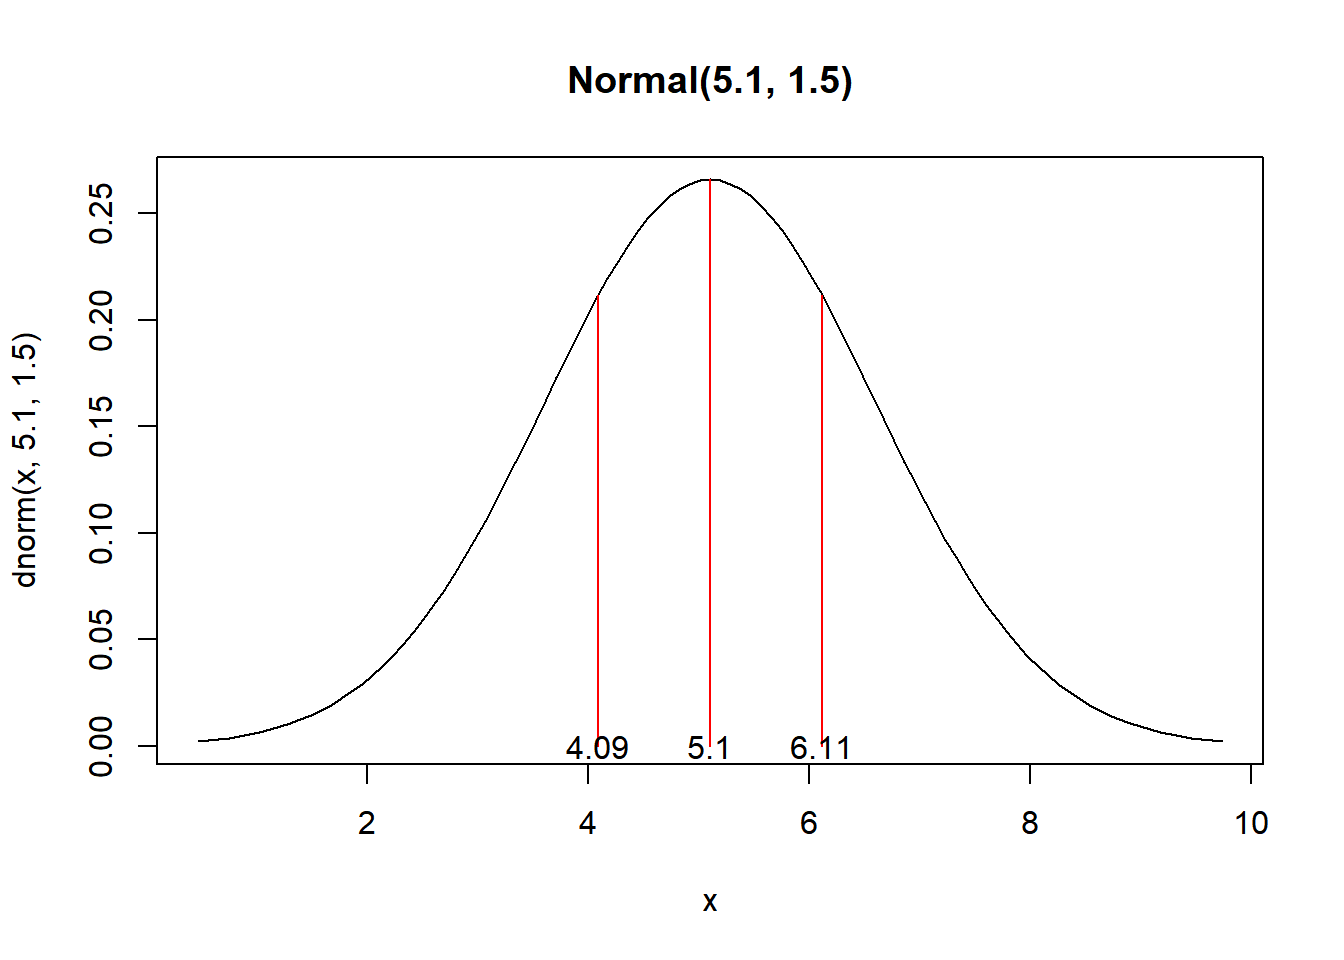
\includegraphics{2_Variable_Aleatoria_Ejercicio_Plantilla_files/figure-latex/unnamed-chunk-31-1.pdf}

\begin{itemize}
\tightlist
\item
  La probabilidad \(P [X > 2]\) como área bajo la función de densidad.
\end{itemize}

\begin{Shaded}
\begin{Highlighting}[]
\CommentTok{# Responde aquí}
\CommentTok{# Primero representamos lo que estamos calculando}
\NormalTok{a <-}\StringTok{ }\DecValTok{2} \CommentTok{# Extremo inferior}
\NormalTok{b <-}\StringTok{ }\KeywordTok{qexp}\NormalTok{(}\FloatTok{0.99}\NormalTok{, }\DecValTok{1}\OperatorTok{/}\DecValTok{2}\NormalTok{) }\CommentTok{# Extremo superior}
\NormalTok{cord.x <-}\StringTok{ }\KeywordTok{c}\NormalTok{(a, }\KeywordTok{seq}\NormalTok{(a, b, }\FloatTok{0.01}\NormalTok{), b) }
\NormalTok{cord.y <-}\StringTok{ }\KeywordTok{c}\NormalTok{(}\DecValTok{0}\NormalTok{, }\KeywordTok{dexp}\NormalTok{(}\KeywordTok{seq}\NormalTok{(a, b, }\FloatTok{0.01}\NormalTok{), }\DecValTok{1}\OperatorTok{/}\DecValTok{2}\NormalTok{), }\DecValTok{0}\NormalTok{) }
\KeywordTok{curve}\NormalTok{(}\KeywordTok{dexp}\NormalTok{(x, }\DecValTok{1}\OperatorTok{/}\DecValTok{2}\NormalTok{), }\DataTypeTok{xlim =} \KeywordTok{c}\NormalTok{(}\DecValTok{0}\NormalTok{, }\KeywordTok{qexp}\NormalTok{(}\FloatTok{0.99}\NormalTok{, }\DecValTok{1}\OperatorTok{/}\DecValTok{2}\NormalTok{)), }\DataTypeTok{main =} \StringTok{'exp(2)'}\NormalTok{)}
\KeywordTok{polygon}\NormalTok{(cord.x, cord.y, }\DataTypeTok{col =} \StringTok{'red'}\NormalTok{)}
\end{Highlighting}
\end{Shaded}

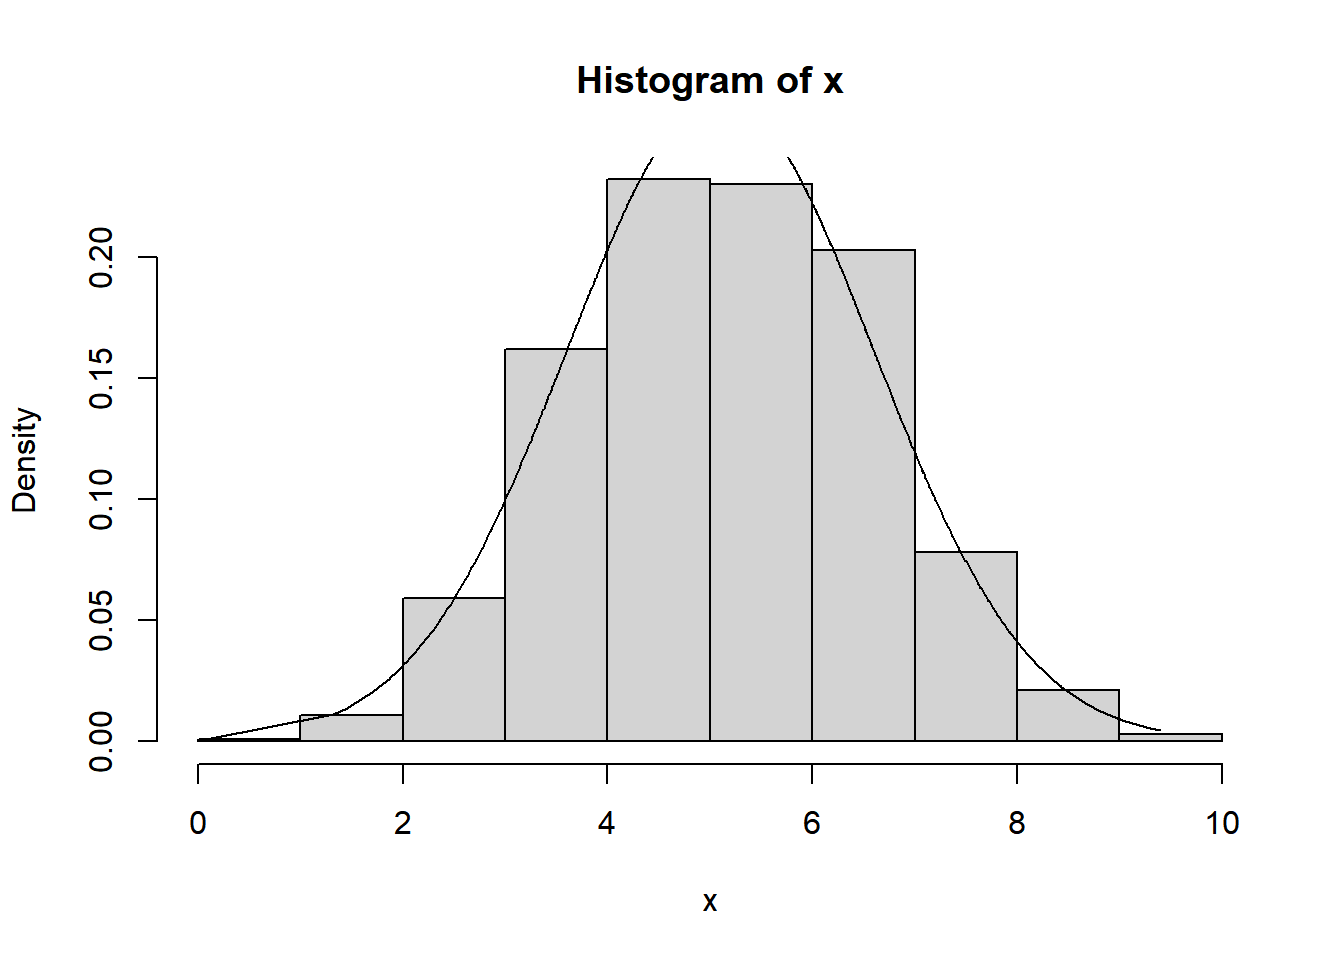
\includegraphics{2_Variable_Aleatoria_Ejercicio_Plantilla_files/figure-latex/unnamed-chunk-32-1.pdf}

\begin{itemize}
\tightlist
\item
  La probabilidad \(P [X = 2]\) como área bajo la función de densidad.
\end{itemize}

\begin{Shaded}
\begin{Highlighting}[]
\CommentTok{# Responde aquí}
\NormalTok{a <-}\StringTok{ }\DecValTok{2} \CommentTok{# Extremo inferior}
\NormalTok{b <-}\StringTok{ }\DecValTok{2} \CommentTok{# Extremo superior (obviamente no ponemos infinito, sino un valor alto de la distribución)}
\NormalTok{cord.x <-}\StringTok{ }\KeywordTok{c}\NormalTok{(a, }\KeywordTok{seq}\NormalTok{(a, b, }\FloatTok{0.01}\NormalTok{), b) }
\NormalTok{cord.y <-}\StringTok{ }\KeywordTok{c}\NormalTok{(}\DecValTok{0}\NormalTok{, }\KeywordTok{dexp}\NormalTok{(}\KeywordTok{seq}\NormalTok{(a, b, }\FloatTok{0.01}\NormalTok{), }\DecValTok{1}\OperatorTok{/}\DecValTok{2}\NormalTok{), }\DecValTok{0}\NormalTok{) }
\KeywordTok{curve}\NormalTok{(}\KeywordTok{dexp}\NormalTok{(x, }\DecValTok{1}\OperatorTok{/}\DecValTok{2}\NormalTok{), }\DataTypeTok{xlim =} \KeywordTok{c}\NormalTok{(}\DecValTok{0}\NormalTok{, }\KeywordTok{qexp}\NormalTok{(}\FloatTok{0.99}\NormalTok{, }\DecValTok{1}\OperatorTok{/}\DecValTok{2}\NormalTok{)), }\DataTypeTok{main =} \StringTok{'exp(2)'}\NormalTok{) }
\KeywordTok{polygon}\NormalTok{(cord.x, cord.y, }\DataTypeTok{col =} \StringTok{'red'}\NormalTok{)}
\end{Highlighting}
\end{Shaded}

\includegraphics{2_Variable_Aleatoria_Ejercicio_Plantilla_files/figure-latex/unnamed-chunk-33-1.pdf}

\hypertarget{cuarto-ejercicio}{%
\section{Cuarto ejercicio}\label{cuarto-ejercicio}}

Consideremos una variable aleatoria \(W\) con distribución
\(Normal(250, 13)\). Se pide:

\begin{enumerate}
\def\labelenumi{\arabic{enumi}.}
\tightlist
\item
  Calcular:
\end{enumerate}

\begin{itemize}
\tightlist
\item
  \(P[240 \leq W < 250]\).
\end{itemize}

\begin{Shaded}
\begin{Highlighting}[]
\CommentTok{# Responde aquí}
\KeywordTok{pnorm}\NormalTok{(}\DecValTok{250}\NormalTok{,}\DecValTok{250}\NormalTok{,}\DecValTok{13}\NormalTok{)}\OperatorTok{-}\KeywordTok{pnorm}\NormalTok{(}\DecValTok{240}\NormalTok{,}\DecValTok{250}\NormalTok{,}\DecValTok{13}\NormalTok{)}
\end{Highlighting}
\end{Shaded}

\begin{verbatim}
## [1] 0.2791218
\end{verbatim}

\begin{itemize}
\tightlist
\item
  \(P[240 < W \leq 250]\).
\end{itemize}

\begin{Shaded}
\begin{Highlighting}[]
\CommentTok{# Responde aquí}
\KeywordTok{pnorm}\NormalTok{(}\DecValTok{250}\NormalTok{,}\DecValTok{250}\NormalTok{,}\DecValTok{13}\NormalTok{)}\OperatorTok{-}\KeywordTok{pnorm}\NormalTok{(}\DecValTok{240}\NormalTok{,}\DecValTok{250}\NormalTok{,}\DecValTok{13}\NormalTok{)}
\end{Highlighting}
\end{Shaded}

\begin{verbatim}
## [1] 0.2791218
\end{verbatim}

\begin{itemize}
\tightlist
\item
  \(P [W > 271]\).
\end{itemize}

\begin{Shaded}
\begin{Highlighting}[]
\CommentTok{# Responde aquí}
\DecValTok{1}\OperatorTok{-}\KeywordTok{pnorm}\NormalTok{(}\DecValTok{271}\NormalTok{,}\DecValTok{250}\NormalTok{,}\DecValTok{13}\NormalTok{)}
\end{Highlighting}
\end{Shaded}

\begin{verbatim}
## [1] 0.05311371
\end{verbatim}

\begin{itemize}
\tightlist
\item
  \(P [W < 271]\).
\end{itemize}

\begin{Shaded}
\begin{Highlighting}[]
\CommentTok{# Responde aquí}
\KeywordTok{pnorm}\NormalTok{(}\DecValTok{271}\NormalTok{,}\DecValTok{250}\NormalTok{,}\DecValTok{13}\NormalTok{)}
\end{Highlighting}
\end{Shaded}

\begin{verbatim}
## [1] 0.9468863
\end{verbatim}

\begin{itemize}
\tightlist
\item
  \(P [W = 271]\).
\end{itemize}

\begin{Shaded}
\begin{Highlighting}[]
\CommentTok{# Responde aquí}
\KeywordTok{pnorm}\NormalTok{(}\DecValTok{271}\NormalTok{,}\DecValTok{250}\NormalTok{,}\DecValTok{13}\NormalTok{)}\OperatorTok{-}\KeywordTok{pnorm}\NormalTok{(}\DecValTok{271}\NormalTok{,}\DecValTok{250}\NormalTok{,}\DecValTok{13}\NormalTok{)}
\end{Highlighting}
\end{Shaded}

\begin{verbatim}
## [1] 0
\end{verbatim}

\begin{enumerate}
\def\labelenumi{\arabic{enumi}.}
\setcounter{enumi}{1}
\tightlist
\item
  Obtener:
\end{enumerate}

\begin{itemize}
\tightlist
\item
  El intervalo de valores de la variable que excluye el 5\% de los
  valores más altos de la distribución y el 5\% de valores más bajos.
\end{itemize}

\begin{Shaded}
\begin{Highlighting}[]
\CommentTok{# Responde aquí}
\KeywordTok{qnorm}\NormalTok{(}\KeywordTok{c}\NormalTok{(}\FloatTok{0.95}\NormalTok{,}\FloatTok{0.05}\NormalTok{),}\DecValTok{250}\NormalTok{,}\DecValTok{13}\NormalTok{)}
\end{Highlighting}
\end{Shaded}

\begin{verbatim}
## [1] 271.3831 228.6169
\end{verbatim}

\begin{enumerate}
\def\labelenumi{\arabic{enumi}.}
\setcounter{enumi}{2}
\tightlist
\item
  Obtener una muestra de tamaño 10 de la distribución.
\end{enumerate}

\begin{Shaded}
\begin{Highlighting}[]
\CommentTok{# Responde aquí}
\KeywordTok{rnorm}\NormalTok{(}\DecValTok{10}\NormalTok{,}\DecValTok{250}\NormalTok{,}\DecValTok{13}\NormalTok{)}
\end{Highlighting}
\end{Shaded}

\begin{verbatim}
##  [1] 274.6258 274.2102 238.9349 238.4904 259.9014 245.4019 260.2110 254.5734
##  [9] 273.8898 242.1466
\end{verbatim}

\begin{enumerate}
\def\labelenumi{\arabic{enumi}.}
\setcounter{enumi}{3}
\tightlist
\item
  Representar:
\end{enumerate}

\begin{itemize}
\tightlist
\item
  La probabilidad \(P [W > 271]\) como área bajo la función de densidad.
\end{itemize}

\begin{Shaded}
\begin{Highlighting}[]
\CommentTok{# Responde aquí}
\CommentTok{# Primero representamos lo que estamos calculando}
\NormalTok{a <-}\StringTok{ }\DecValTok{271} \CommentTok{# Extremo inferior}
\NormalTok{b <-}\StringTok{ }\KeywordTok{qnorm}\NormalTok{(}\FloatTok{0.999}\NormalTok{, }\DecValTok{250}\NormalTok{,}\DecValTok{13}\NormalTok{) }\CommentTok{# Extremo superior (obviamente no ponemos infinito, sino un valor alto de la distribución)}
\NormalTok{cord.x <-}\StringTok{ }\KeywordTok{c}\NormalTok{(a, }\KeywordTok{seq}\NormalTok{(a, b, }\FloatTok{0.01}\NormalTok{), b) }
\NormalTok{cord.y <-}\StringTok{ }\KeywordTok{c}\NormalTok{(}\DecValTok{0}\NormalTok{, }\KeywordTok{dnorm}\NormalTok{(}\KeywordTok{seq}\NormalTok{(a, b, }\FloatTok{0.01}\NormalTok{), }\DecValTok{250}\NormalTok{,}\DecValTok{13}\NormalTok{), }\DecValTok{0}\NormalTok{) }
\KeywordTok{curve}\NormalTok{(}\KeywordTok{dnorm}\NormalTok{(x, }\DecValTok{250}\NormalTok{,}\DecValTok{13}\NormalTok{), }\DataTypeTok{xlim =} \KeywordTok{qnorm}\NormalTok{(}\KeywordTok{c}\NormalTok{(}\FloatTok{0.001}\NormalTok{, }\FloatTok{0.999}\NormalTok{),}\DecValTok{250}\NormalTok{,}\DecValTok{13}\NormalTok{), }\DataTypeTok{main =} \StringTok{'Normal(250, 13)'}\NormalTok{) }
\KeywordTok{polygon}\NormalTok{(cord.x, cord.y, }\DataTypeTok{col =} \StringTok{'red'}\NormalTok{)}
\end{Highlighting}
\end{Shaded}

\includegraphics{2_Variable_Aleatoria_Ejercicio_Plantilla_files/figure-latex/unnamed-chunk-41-1.pdf}

\begin{itemize}
\tightlist
\item
  La probabilidad \(P [W < 271]\) como área bajo la función de densidad.
\end{itemize}

\begin{Shaded}
\begin{Highlighting}[]
\CommentTok{# Responde aquí}
\CommentTok{# Primero representamos lo que estamos calculando}
\NormalTok{a <-}\StringTok{ }\KeywordTok{qnorm}\NormalTok{(}\FloatTok{0.001}\NormalTok{, }\DecValTok{250}\NormalTok{,}\DecValTok{13}\NormalTok{) }\CommentTok{# Extremo inferior}
\NormalTok{b <-}\StringTok{ }\DecValTok{271} \CommentTok{# Extremo superior (obviamente no ponemos infinito, sino un valor alto de la distribución)}
\NormalTok{cord.x <-}\StringTok{ }\KeywordTok{c}\NormalTok{(a, }\KeywordTok{seq}\NormalTok{(a, b, }\FloatTok{0.01}\NormalTok{), b) }
\NormalTok{cord.y <-}\StringTok{ }\KeywordTok{c}\NormalTok{(}\DecValTok{0}\NormalTok{, }\KeywordTok{dnorm}\NormalTok{(}\KeywordTok{seq}\NormalTok{(a, b, }\FloatTok{0.01}\NormalTok{), }\DecValTok{250}\NormalTok{,}\DecValTok{13}\NormalTok{), }\DecValTok{0}\NormalTok{) }
\KeywordTok{curve}\NormalTok{(}\KeywordTok{dnorm}\NormalTok{(x, }\DecValTok{250}\NormalTok{,}\DecValTok{13}\NormalTok{), }\DataTypeTok{xlim =} \KeywordTok{qnorm}\NormalTok{(}\KeywordTok{c}\NormalTok{(}\FloatTok{0.001}\NormalTok{, }\FloatTok{0.999}\NormalTok{),}\DecValTok{250}\NormalTok{,}\DecValTok{13}\NormalTok{), }\DataTypeTok{main =} \StringTok{'Normal(250, 13)'}\NormalTok{) }
\KeywordTok{polygon}\NormalTok{(cord.x, cord.y, }\DataTypeTok{col =} \StringTok{'red'}\NormalTok{)}
\end{Highlighting}
\end{Shaded}

\includegraphics{2_Variable_Aleatoria_Ejercicio_Plantilla_files/figure-latex/unnamed-chunk-42-1.pdf}

\begin{itemize}
\tightlist
\item
  La probabilidad \(P [W \leq 271]\) como área bajo la función de
  densidad.
\end{itemize}

\begin{Shaded}
\begin{Highlighting}[]
\CommentTok{# Responde aquí}
\CommentTok{# Primero representamos lo que estamos calculando}
\NormalTok{a <-}\StringTok{ }\KeywordTok{qnorm}\NormalTok{(}\FloatTok{0.001}\NormalTok{, }\DecValTok{250}\NormalTok{,}\DecValTok{13}\NormalTok{) }\CommentTok{# Extremo inferior}
\NormalTok{b <-}\StringTok{ }\DecValTok{271} \CommentTok{# Extremo superior (obviamente no ponemos infinito, sino un valor alto de la distribución)}
\NormalTok{cord.x <-}\StringTok{ }\KeywordTok{c}\NormalTok{(a, }\KeywordTok{seq}\NormalTok{(a, b, }\FloatTok{0.01}\NormalTok{), b) }
\NormalTok{cord.y <-}\StringTok{ }\KeywordTok{c}\NormalTok{(}\DecValTok{0}\NormalTok{, }\KeywordTok{dnorm}\NormalTok{(}\KeywordTok{seq}\NormalTok{(a, b, }\FloatTok{0.01}\NormalTok{), }\DecValTok{250}\NormalTok{,}\DecValTok{13}\NormalTok{), }\DecValTok{0}\NormalTok{) }
\KeywordTok{curve}\NormalTok{(}\KeywordTok{dnorm}\NormalTok{(x, }\DecValTok{250}\NormalTok{,}\DecValTok{13}\NormalTok{), }\DataTypeTok{xlim =} \KeywordTok{qnorm}\NormalTok{(}\KeywordTok{c}\NormalTok{(}\FloatTok{0.001}\NormalTok{, }\FloatTok{0.999}\NormalTok{),}\DecValTok{250}\NormalTok{,}\DecValTok{13}\NormalTok{), }\DataTypeTok{main =} \StringTok{'Normal(250, 13)'}\NormalTok{) }
\KeywordTok{polygon}\NormalTok{(cord.x, cord.y, }\DataTypeTok{col =} \StringTok{'red'}\NormalTok{)}
\end{Highlighting}
\end{Shaded}

\includegraphics{2_Variable_Aleatoria_Ejercicio_Plantilla_files/figure-latex/unnamed-chunk-43-1.pdf}

\begin{itemize}
\tightlist
\item
  La probabilidad \(P [W = 271]\) como área bajo la función de densidad.
\end{itemize}

\begin{Shaded}
\begin{Highlighting}[]
\CommentTok{# Responde aquí}
\CommentTok{# Primero representamos lo que estamos calculando}
\NormalTok{a <-}\StringTok{ }\DecValTok{271} \CommentTok{# Extremo inferior}
\NormalTok{b <-}\StringTok{ }\DecValTok{271} \CommentTok{# Extremo superior (obviamente no ponemos infinito, sino un valor alto de la distribución)}
\NormalTok{cord.x <-}\StringTok{ }\KeywordTok{c}\NormalTok{(a, }\KeywordTok{seq}\NormalTok{(a, b, }\FloatTok{0.01}\NormalTok{), b) }
\NormalTok{cord.y <-}\StringTok{ }\KeywordTok{c}\NormalTok{(}\DecValTok{0}\NormalTok{, }\KeywordTok{dnorm}\NormalTok{(}\KeywordTok{seq}\NormalTok{(a, b, }\FloatTok{0.01}\NormalTok{), }\DecValTok{250}\NormalTok{,}\DecValTok{13}\NormalTok{), }\DecValTok{0}\NormalTok{) }
\KeywordTok{curve}\NormalTok{(}\KeywordTok{dnorm}\NormalTok{(x, }\DecValTok{250}\NormalTok{,}\DecValTok{13}\NormalTok{), }\DataTypeTok{xlim =} \KeywordTok{qnorm}\NormalTok{(}\KeywordTok{c}\NormalTok{(}\FloatTok{0.001}\NormalTok{, }\FloatTok{0.999}\NormalTok{),}\DecValTok{250}\NormalTok{,}\DecValTok{13}\NormalTok{), }\DataTypeTok{main =} \StringTok{'Normal(250, 13)'}\NormalTok{) }
\KeywordTok{polygon}\NormalTok{(cord.x, cord.y, }\DataTypeTok{col =} \StringTok{'red'}\NormalTok{)}
\end{Highlighting}
\end{Shaded}

\includegraphics{2_Variable_Aleatoria_Ejercicio_Plantilla_files/figure-latex/unnamed-chunk-44-1.pdf}

\end{document}
